\begin{frame}
    \frametitle{Đơn cực từ}
    Xét sự chuyển động của một điện tích điểm \(q_e\), khối lượng \(m\) trong từ trường của một đơn cực từ giả tưởng nằm yên tại gốc toạ độ:
    \[\mathbf{B}=k\frac{q_m}{r^2}\hat{r}.\]
    \begin{itemize}
        \item Phương trình động lực học: \(m\mathbf{a}=q_e(\mathbf{v}\times\mathbf{B})\).
        \item Công suất của lực từ bằng 0: \(\lvert\mathbf{v}\rvert=const\).
    \end{itemize}
    Chứng minh được rằng, đại lượng \[\mathbf{Q}=\mathbf{L}-kq_e q_m \hat{r}\] là một hằng số chuyển động (bất biến).
\end{frame}
\begin{frame}
    \frametitle{Đơn cực từ}
    \begin{columns}
        \begin{column}{0.5\textwidth}
            \vspace{-16pt}

            \begin{figure}
        \centering
        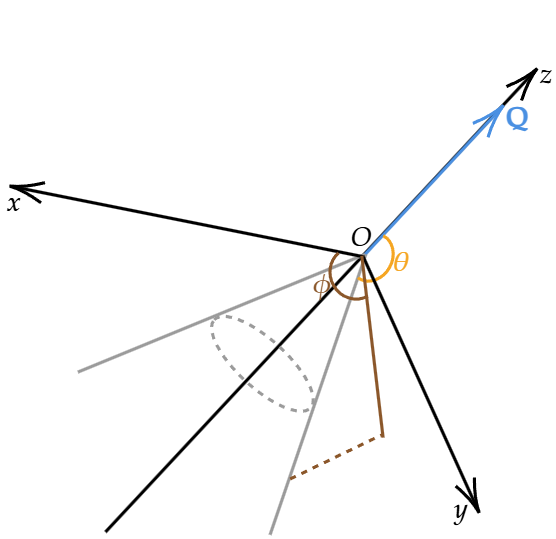
\includegraphics[width=6cm, height=6cm]{Content/Figure/magnetic_monopole.png}
    \end{figure}
        \end{column}
        \begin{column}{0.5\textwidth}
            \begin{itemize}
                \item \(\mathbf{Q}\cdot\hat{\phi}=mr^2\dot\theta=0\implies \theta=const\).
                \item \(\mathbf{Q}\cdot\hat{r}=Q\cos\theta=-kq_e q_m \implies \lvert \mathbf{Q}\rvert =const\).
                \item \(r(\phi)=\frac{Q\sin\theta}{mv\cos((\phi-\phi_0)\sin\theta)}\).
            \end{itemize}
            
        \end{column}
    \end{columns}
\end{frame}

\begin{frame}
\frametitle{Bất biến đoạn nhiệt}
Một vật nhỏ có khối lượng \(m\) chuyển động và va chạm đàn hồi với hai vạch tường cách nhau một khoảng \(L\). Dịch chuyển vách tường bên phải lại một cách rất chậm. Tìm liên hệ giữa vận tốc \(v\) của vật và độ dịch chuyển \(x\) của tường.
\begin{figure}
    \centering
    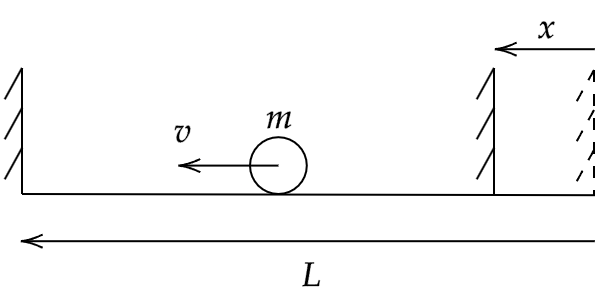
\includegraphics[width=0.5\textwidth]{Content/Figure/adiabatic.png}
\end{figure}
\end{frame}

\begin{frame}
\frametitle{Bất biến đoạn nhiệt}
Sau mỗi va chạm, tường truyền cho vật một động lượng \(\Delta p = 2mv\).

Tường giống như tác dụng một "lực" \(F\) lên vật:
\begin{equation*}
    F=\frac{\Delta p}{\Delta t}=\frac{2mv}{\frac{2(L-x)}{v}}.
\end{equation*}
Định lí công - động năng:
\begin{equation*}
    d\left(\frac{mv^2}{2}\right)=F dx=\frac{mv^2}{L-x}dx.
\end{equation*}
Chuyển vế và nguyên hàm, ta thu được:
\begin{equation}
    v(L-x)=const.
\end{equation}
\end{frame}
\begin{frame}
    \frametitle{Một ``nghịch lý''}
    Một quả tên lửa có thể cung cấp vận tốc \(u\), tức năng lượng bằng \(\frac{mu^2}{2}\) cho đầu đạn sau khi đốt hết nhiên liệu. Vậy nếu như tên lửa được phóng từ một máy bay đang bay
    với vận tốc \(v\), vận tốc của đầu đạn sẽ là \(v+u\). Như vậy động năng tổng cộng của đầu đạn lúc này là \[\frac{m(v+u)^2}{2}>\frac{mu^2}{2}+\frac{mv^2}{2}.\] Trong khi ta biết rằng tổng hoá năng của nhiên liệu là không đổi trong cả hai trường hợp, vậy lượng năng lượng này từ đâu r? 
    Coi rằng tổng khối lượng của nhiên liệu là rất nhỏ so với khối lượng của đầu đạn.
\end{frame}